\documentclass[aps,jcp,preprint,showpacs,superscriptaddress,groupedaddress]{revtex4}  % for double-spaced preprint
\usepackage{graphicx}  % needed for figures
\usepackage{dcolumn}   % needed for some tables
\usepackage{bm}        % for math
\usepackage{amssymb}   % for math
%\usepackage{booktabs}
\usepackage{multirow}
\usepackage{tablefootnote}
\usepackage{times}
\usepackage{mathptm}
\usepackage[version=3]{mhchem}

\begin{document}

\title{Supporting Information for: \\
The different facets of ice have different hydrophilicities: Friction at water /
  ice-I$_\mathrm{h}$ interfaces}

\author{Patrick B. Louden}
\author{J. Daniel Gezelter}
\email{gezelter@nd.edu}
\affiliation{Department of Chemistry and Biochemistry, University of
  Notre Dame, Notre Dame, IN 46556}

\date{\today}

\begin{abstract}
The supporting information supplies figures that support the data
presented in the main text.
\end{abstract}

\pacs{68.08.Bc, 68.08.De, 66.20.Cy}


\maketitle

\section{The Advancing Contact Angle}
The advancing contact angles for the liquid droplets were computed
using inversion of Eq. (2) in the main text which requires finding the
real roots of a fourth order polynomial,
\begin{equation}
\label{eq:poly}
c_4 \cos^4 \theta + c_3 \cos^3 \theta + c_2 \cos^2 \theta + c_1
\cos \theta + c_0 = 0
\end{equation}
where the coefficients of the polynomial are expressed in terms of the
$z$ coordinate of the center of mass of the liquid droplet relative to
the solid surface, $z = z_\mathrm{cm} - z_\mathrm{surface}$, and a
factor that depends on the initial droplet radius, $k = 2^{-4/3} R_0$.
The coefficients are simple functions of these two quantities,
\begin{align}
c_4 &= z^3 + k^3 \\
c_3 &= 8 z^3 + 8 k^3 \\
c_2 &= 24 z^3 + 18 k^3 \\
c_1 &= 32 z^3 \\
c_0 &= 16 z^3 - 27 k^3 .
\end{align}
Solving for the values of the real roots of this polynomial
(Eq. \ref{eq:poly}) give estimates of the advancing contact angle.
The dynamics of this quantity for each of the four interfaces is shown
in figure 1 below.

\section{Interfacial widths using structural information}
To determine the structural widths of the interfaces under shear, each
of the systems was divided into 100 bins along the $z$-dimension, and
the local tetrahedral order parameter (Eq. 5 in Reference
\citealp{Louden13}) was time-averaged in each bin for the duration of
the shearing simulation.  The spatial dependence of this order
parameter, $q(z)$, is the tetrahedrality profile of the interface.
The lower panels in figures 2-5 show tetrahedrality profiles (in
circles) for each of the four interfaces.  The $q(z)$ function has a
range of $(0,1)$, where a value of unity indicates a perfectly
tetrahedral environment.  The $q(z)$ for the bulk liquid was found to
be $\approx~0.77$, while values of $\approx~0.92$ were more common in
the ice. The tetrahedrality profiles were fit using a hyperbolic
tangent function (see Eq. 6 in Reference \citealp{Louden13}) designed
to smoothly fit the bulk to ice transition while accounting for the
weak thermal gradient. In panels $b$ and $c$ of the same figures, the
resulting thermal and velocity gradients from an imposed kinetic
energy and momentum fluxes can be seen. The vertical dotted lines
traversing these figures indicate the midpoints of the interfaces as
determined by the tetrahedrality profiles.

\section{Interfacial widths using dynamic information}
To determine the dynamic widths of the interfaces under shear, each of
the systems was divided into bins along the $z$-dimension ($\approx$ 3
\AA\ wide) and $C_2(z,t)$ was computed using only those molecules that
were in the bin at the initial time.  To compute these correlation
functions, each of the 0.5 ns simulations was followed by a shorter
200 ps microcanonical (NVE) simulation in which the positions and
orientations of every molecule in the system were recorded every 0.1
ps. 

The time-dependence was fit to a triexponential decay, with three time
constants: $\tau_{short}$, measuring the librational motion of the
water molecules, $\tau_{middle}$, measuring the timescale for breaking
and making of hydrogen bonds, and $\tau_{long}$, corresponding to the
translational motion of the water molecules.  An additional constant
was introduced in the fits to describe molecules in the crystal which
do not experience long-time orientational decay.

In Figures 6-9, the $z$-coordinate profiles for the three decay
constants, $\tau_{short}$, $\tau_{middle}$, and $\tau_{long}$ for the
different interfaces are shown.  (Figures 6 \& 7 are new results,
and Figures 8 \& 9 are updated plots from Ref \citealp{Louden13}.)
In the liquid regions of all four interfaces, we observe
$\tau_{middle}$ and $\tau_{long}$ to have approximately consistent
values of $3-6$ ps and $30-40$ ps, respectively.  Both of these times
increase in value approaching the interface.  Approaching the
interface, we also observe that $\tau_{short}$ decreases from its
liquid-state value of $72-76$ fs.  The approximate values for the
decay constants and the trends approaching the interface match those
reported previously for the basal and prismatic interfaces.

We have estimated the dynamic interfacial width $d_\mathrm{dyn}$ by
fitting the profiles of all the three orientational time constants
with an exponential decay to the bulk-liquid behavior,
\begin{equation}\label{tauFit}
  \tau(z)\approx\tau_{liquid}+(\tau_{wall}-\tau_{liquid})e^{-(z-z_{wall})/d_\mathrm{dyn}}
\end{equation}
where $\tau_{liquid}$ and $\tau_{wall}$ are the liquid and projected
wall values of the decay constants, $z_{wall}$ is the location of the
interface, as measured by the structural order parameter.  These
values are shown in table 1 in the main text. Because the bins must be
quite wide to obtain reasonable profiles of $C_2(z,t)$, the error
estimates for the dynamic widths of the interface are significantly
larger than for the structural widths.  However, all four interfaces
exhibit dynamic widths that are significantly below 1~nm, and are in
reasonable agreement with the structural width above.

\bibliographystyle{aip}
\bibliography{iceWater}

\newpage
%S1: contact angle
\begin{figure}
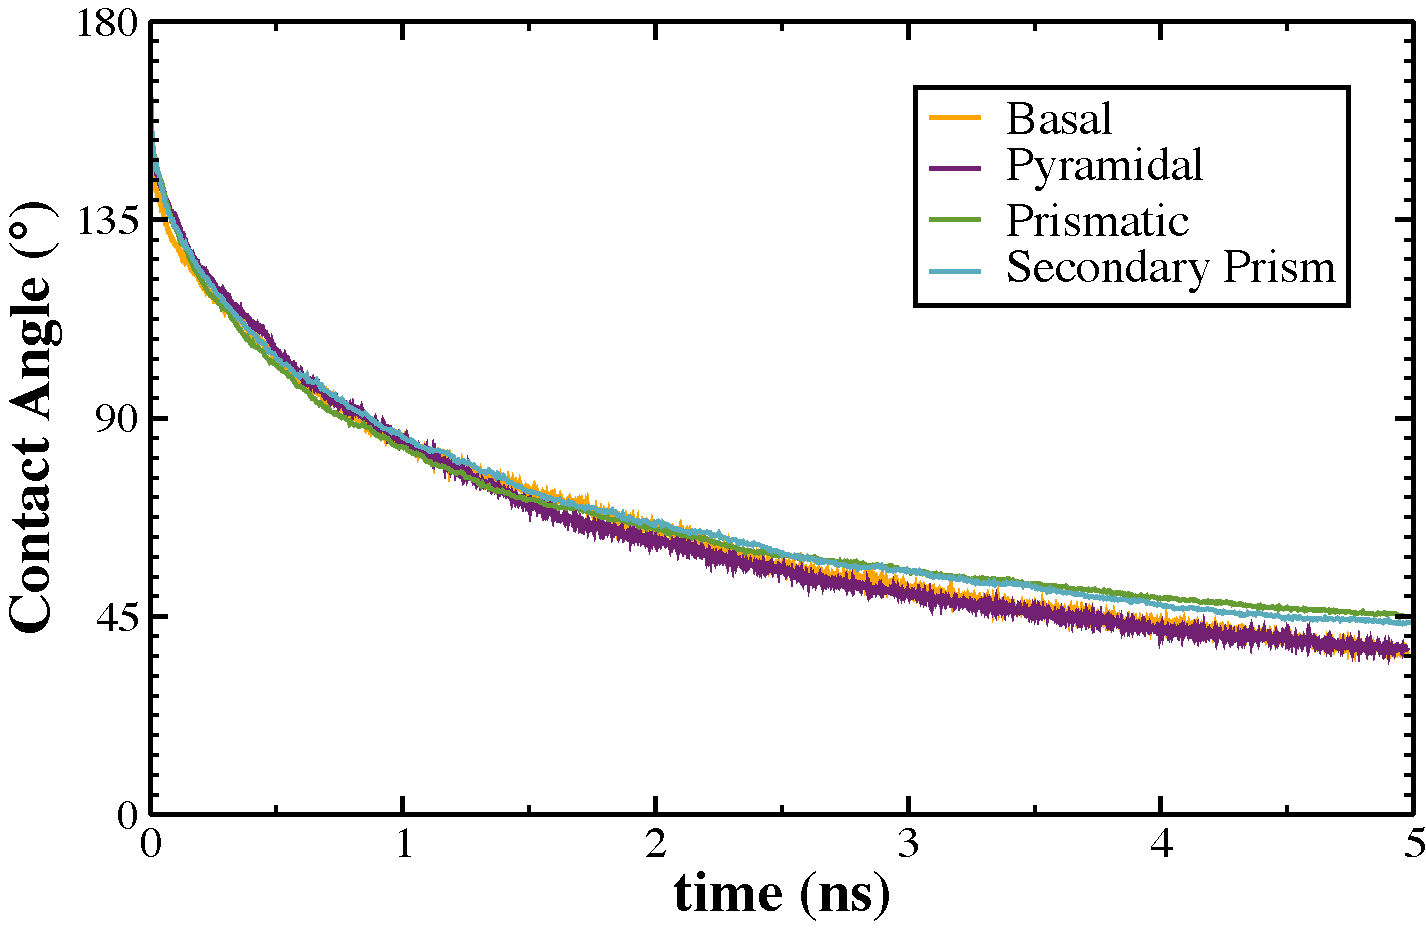
\includegraphics[width=\linewidth]{ContactAngle}
\caption{\label{fig:ContactAngle} The dynamic contact angle of a
  droplet after approaching each of the four ice facets.  The decay to
  an equilibrium contact angle displays similar dynamics.  Although
  all the surfaces are hydrophilic, the long-time behavior stabilizes
  to significantly flatter droplets for the basal and pyramidal
  facets.  This suggests a difference in hydrophilicity for these
  facets compared with the two prismatic facets.}
\end{figure}

\newpage

%S2-S5 are the z-rnemd profiles
\begin{figure}
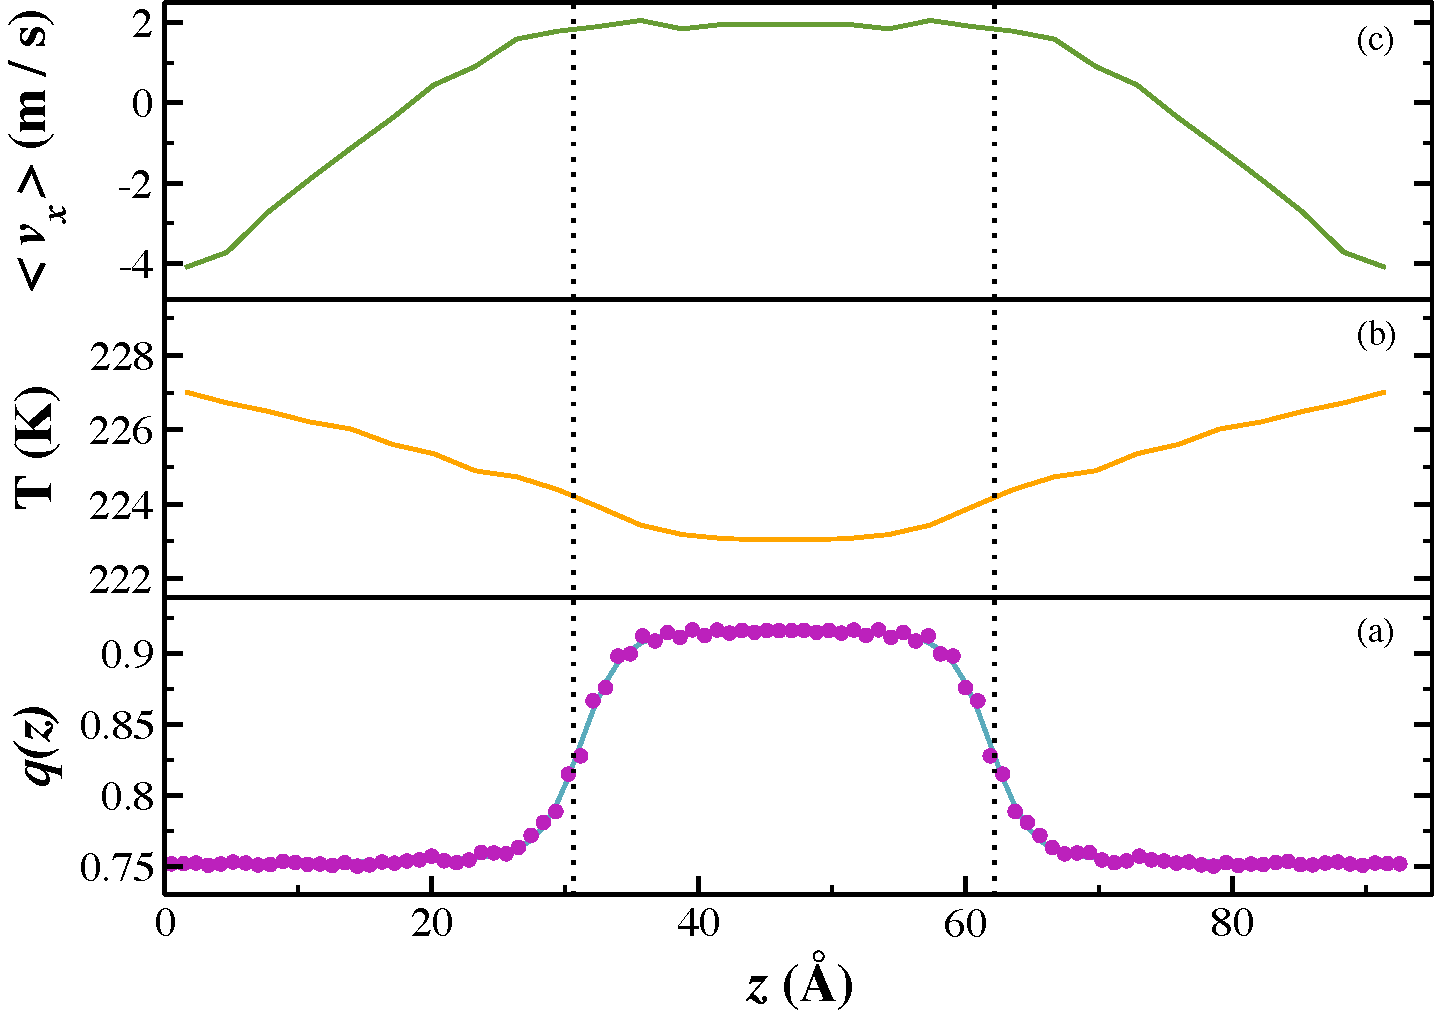
\includegraphics[width=\linewidth]{Pyr_comic_strip}
\caption{\label{fig:pyrComic} Properties of the pyramidal interface
  being sheared through water at 3.8 ms\textsuperscript{-1}. Lower
  panel: the local tetrahedral order parameter, $q(z)$, (circles) and
  the hyperbolic tangent fit (turquoise line).  Middle panel: the
  imposed thermal gradient required to maintain a fixed interfacial
  temperature of 225 K. Upper panel: the transverse velocity gradient
  that develops in response to an imposed momentum flux. The vertical
  dotted lines indicate the locations of the midpoints of the two
  interfaces.}
\end{figure}
\newpage

\begin{figure}
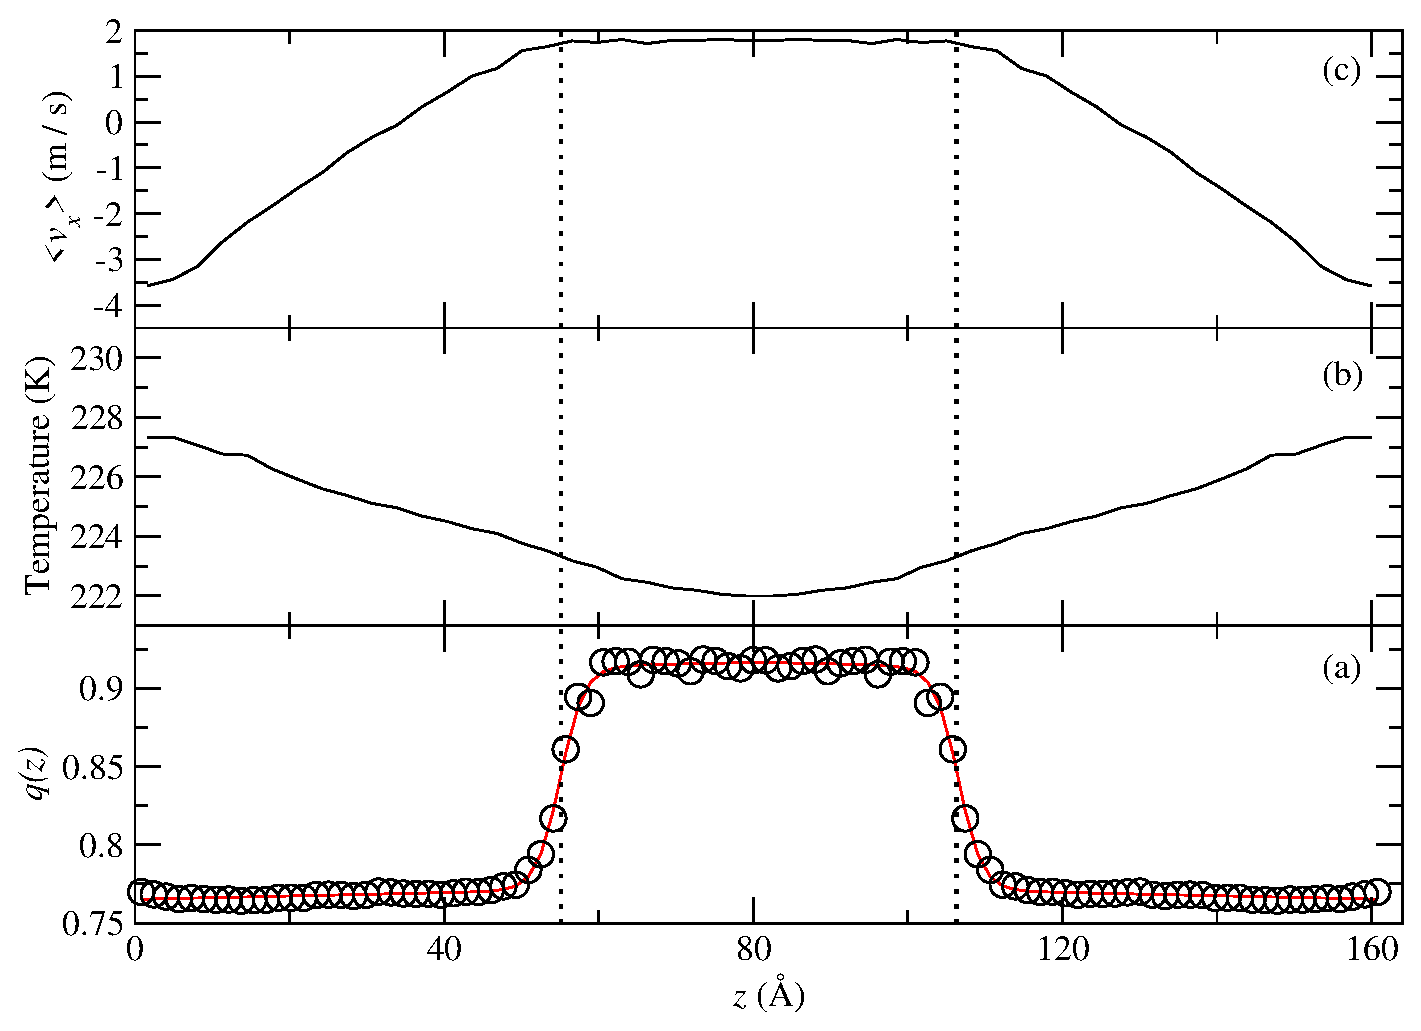
\includegraphics[width=\linewidth]{SP_comic_strip}
\caption{\label{fig:spComic} The secondary prism interface with a shear 
rate of 3.5 \
ms\textsuperscript{-1}. Panel descriptions match those in figure \ref{fig:pyrComic}.}
\end{figure}
\newpage

\begin{figure}
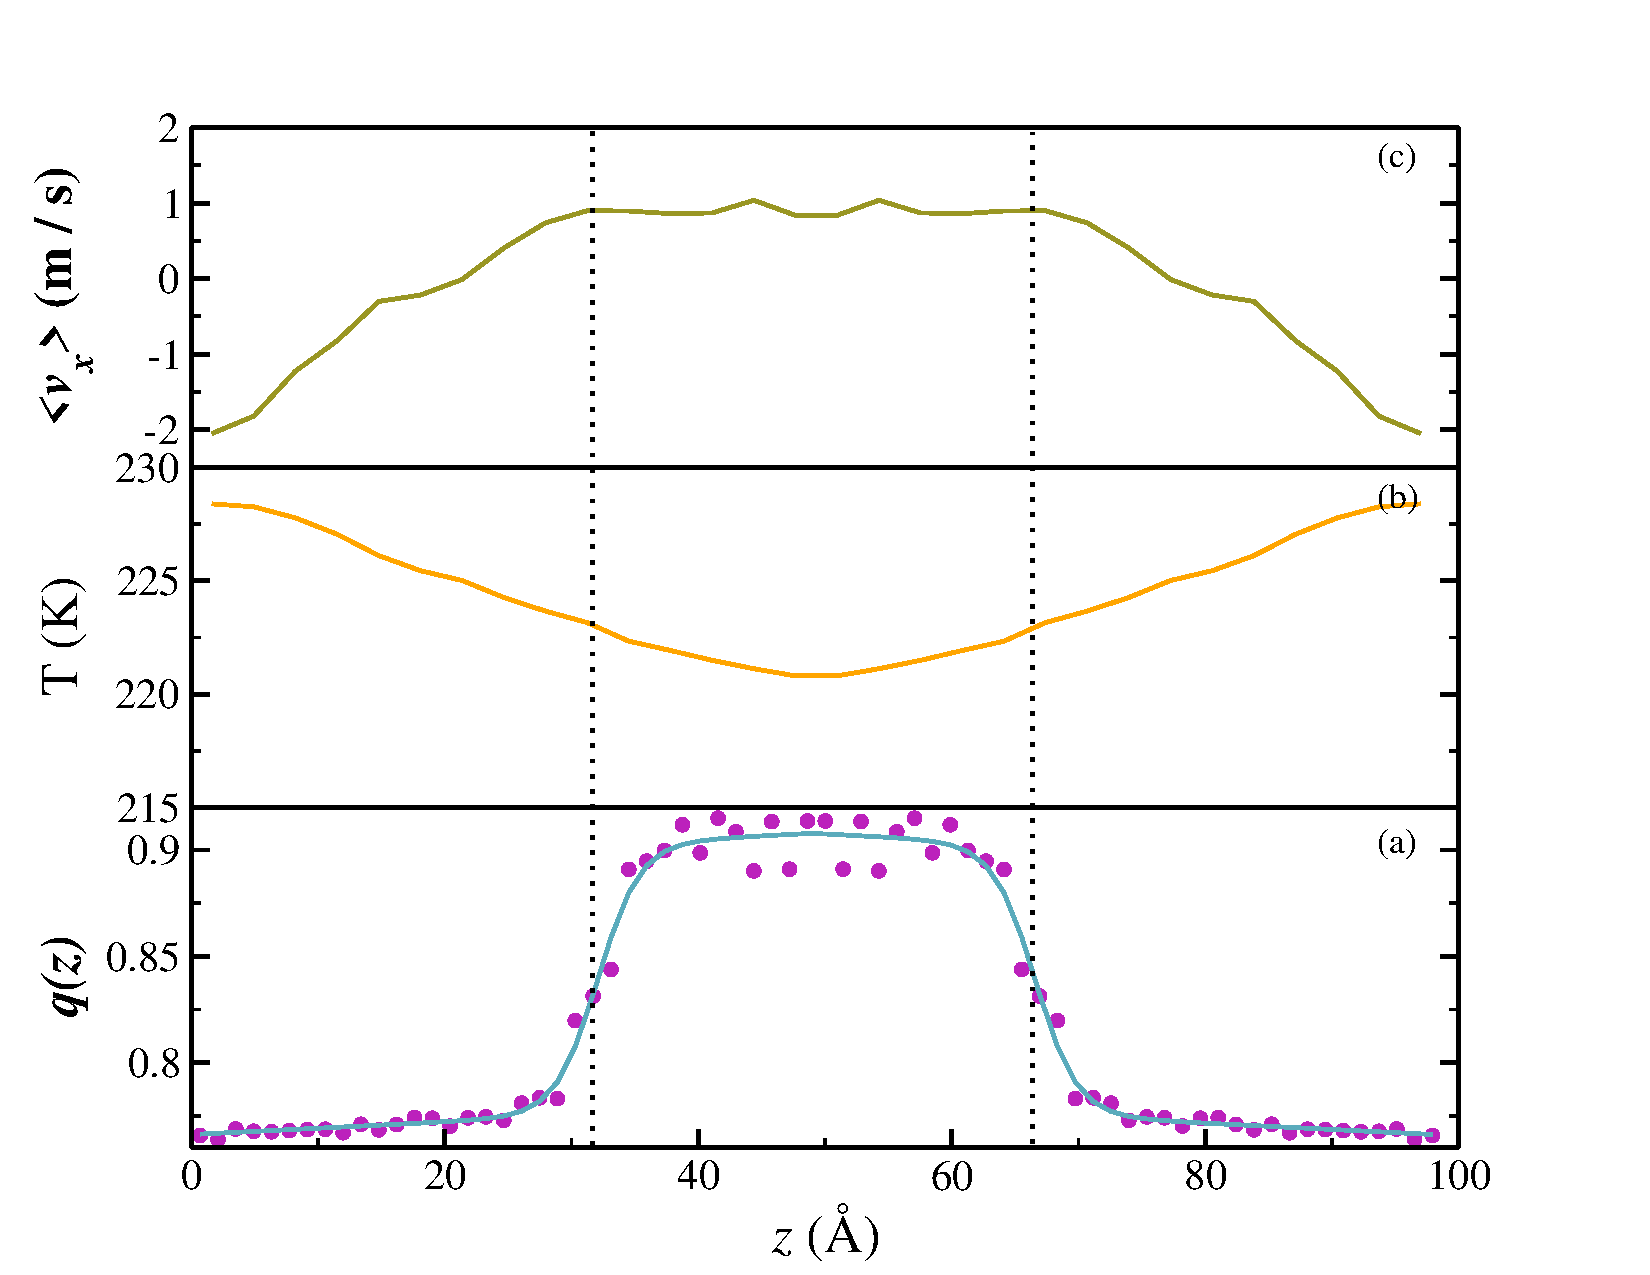
\includegraphics[width=\linewidth]{B_comic_strip}
\caption{\label{fig:bComic} The basal interface with a shear 
rate of 1.3 \
ms\textsuperscript{-1}. Panel descriptions match those in figure \ref{fig:pyrComic}.}
\end{figure}
\newpage

\begin{figure}
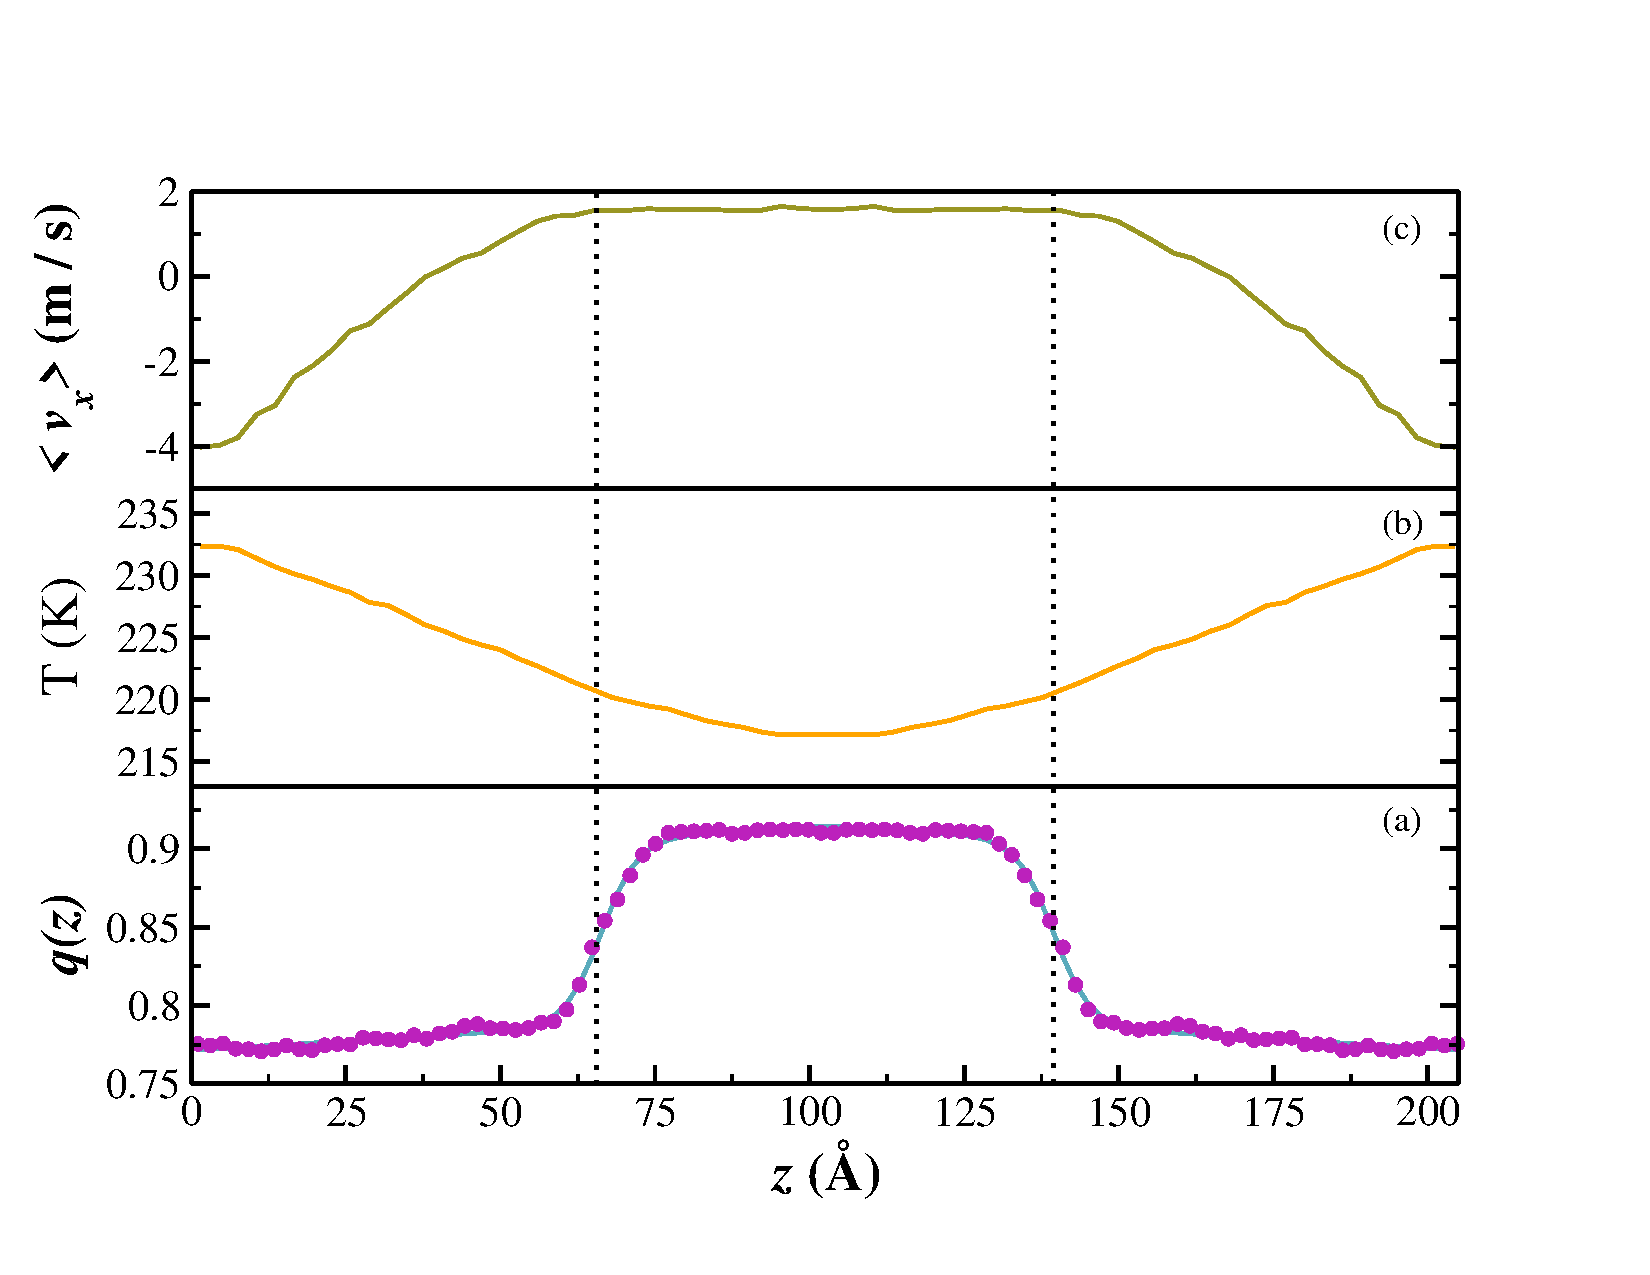
\includegraphics[width=\linewidth]{prismatic_comic_strip}
\caption{\label{fig:pComic} The prismatic interface with a shear 
rate of 2 \
ms\textsuperscript{-1}. Panel descriptions match those in figure \ref{fig:pyrComic}.}
\end{figure}
\newpage

%Figures S6-S9 are the z-orientation times
\begin{figure}
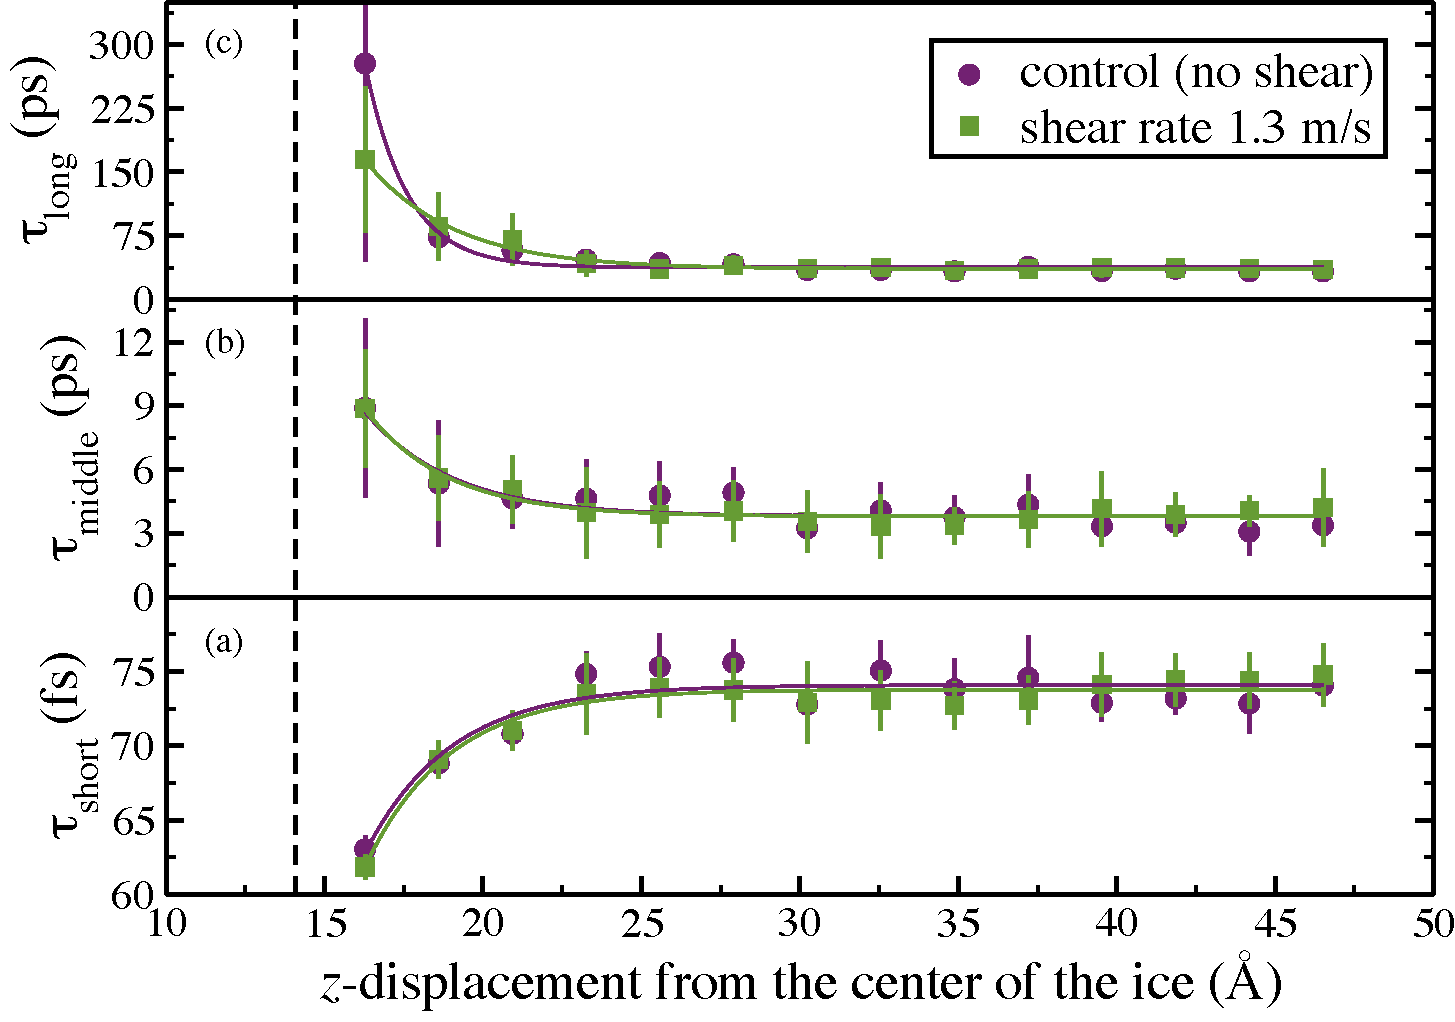
\includegraphics[width=\linewidth]{Pyr-orient}
\caption{\label{fig:PyrOrient} The three decay constants of the
  orientational time correlation function, $C_2(z,t)$, for water as a
  function of distance from the center of the ice slab. The vertical
  dashed line indicates the edge of the pyramidal ice slab determined
  by the local order tetrahedral parameter. The control (circles) and
  sheared (squares) simulations were fit using shifted-exponential
  decay (see Eq. 9 in Ref. \citealp{Louden13}).}
\end{figure}  
\newpage

\begin{figure}
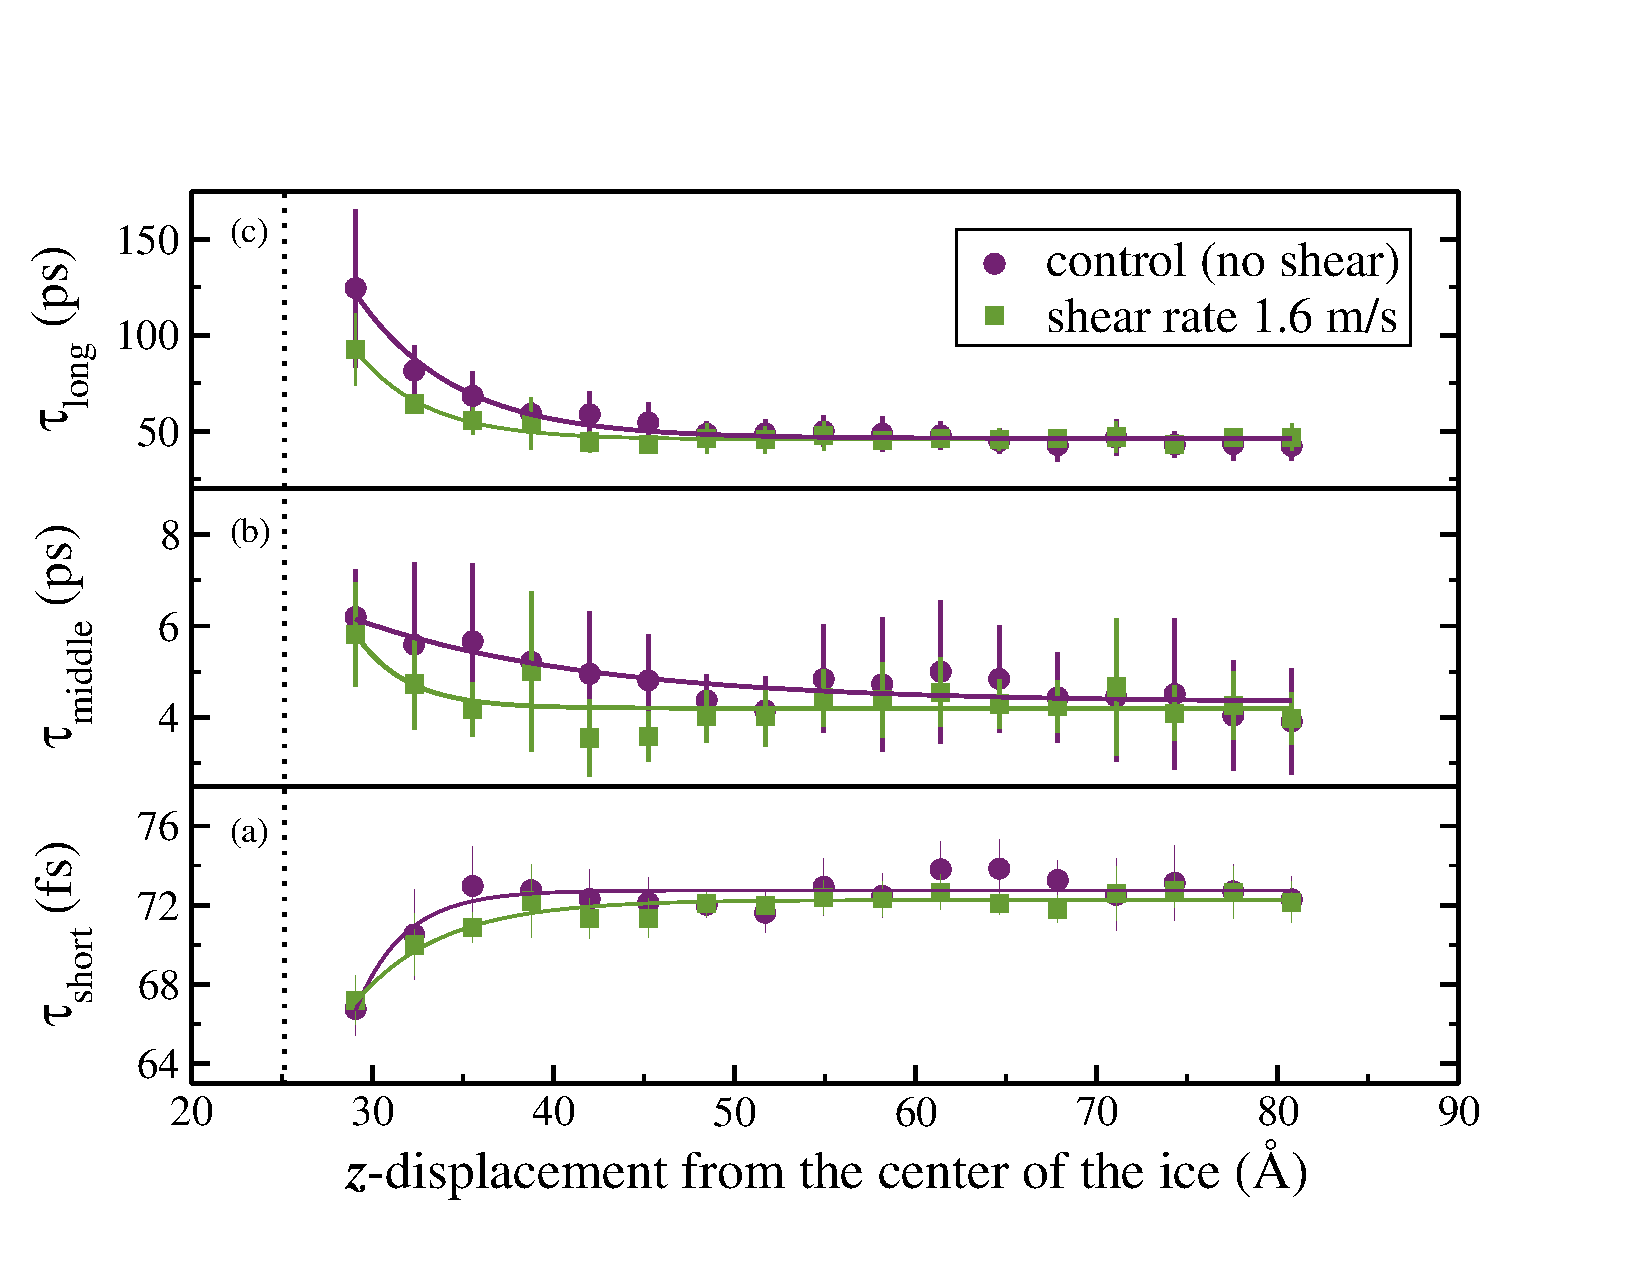
\includegraphics[width=\linewidth]{SP-orient}
\caption{\label{fig:SPorient} Decay constants for $C_2(z,t)$ at the secondary 
prism face. Panel descriptions match those in \ref{fig:PyrOrient}.}
\end{figure}

\newpage

\begin{figure}
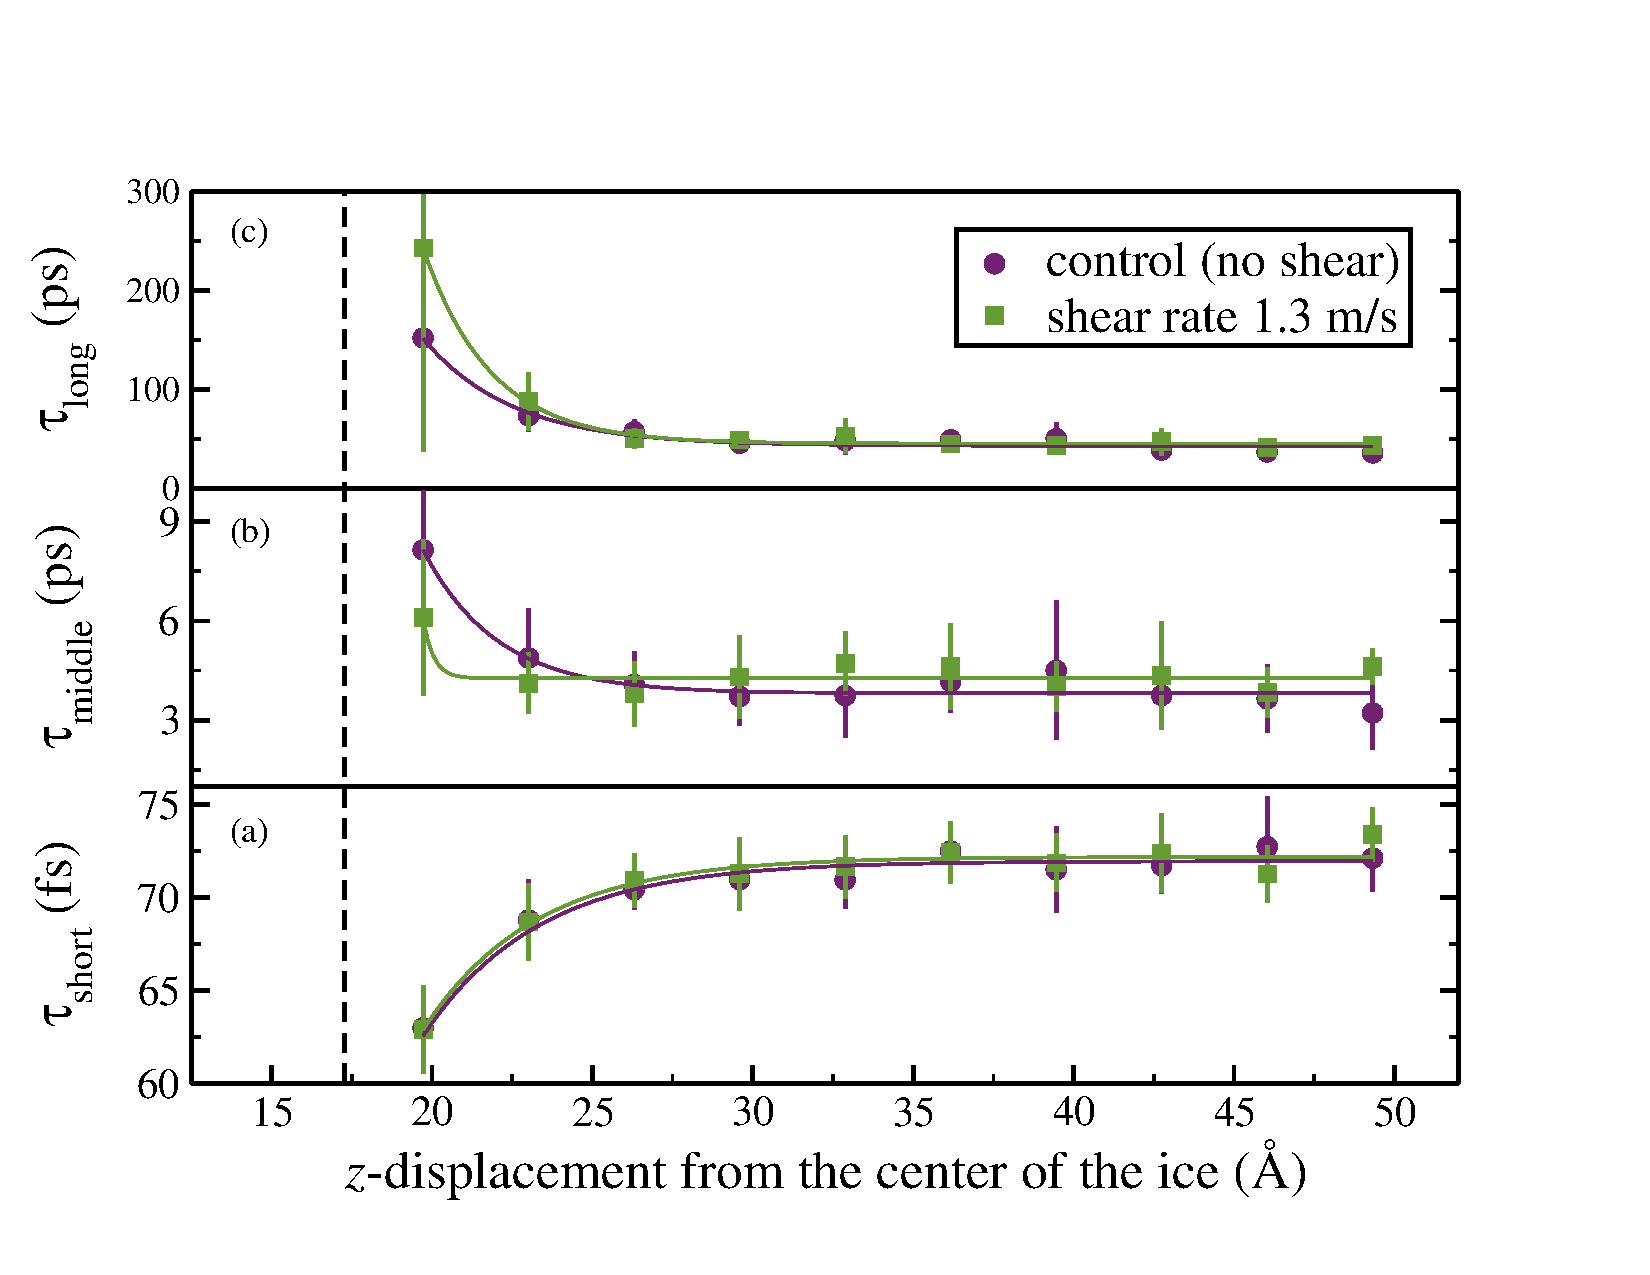
\includegraphics[width=\linewidth]{B-orient}
\caption{\label{fig:Borient} Decay constants for $C_2(z,t)$ at the basal face. Panel descriptions match those in \ref{fig:PyrOrient}.}
\end{figure}
\newpage

\begin{figure}
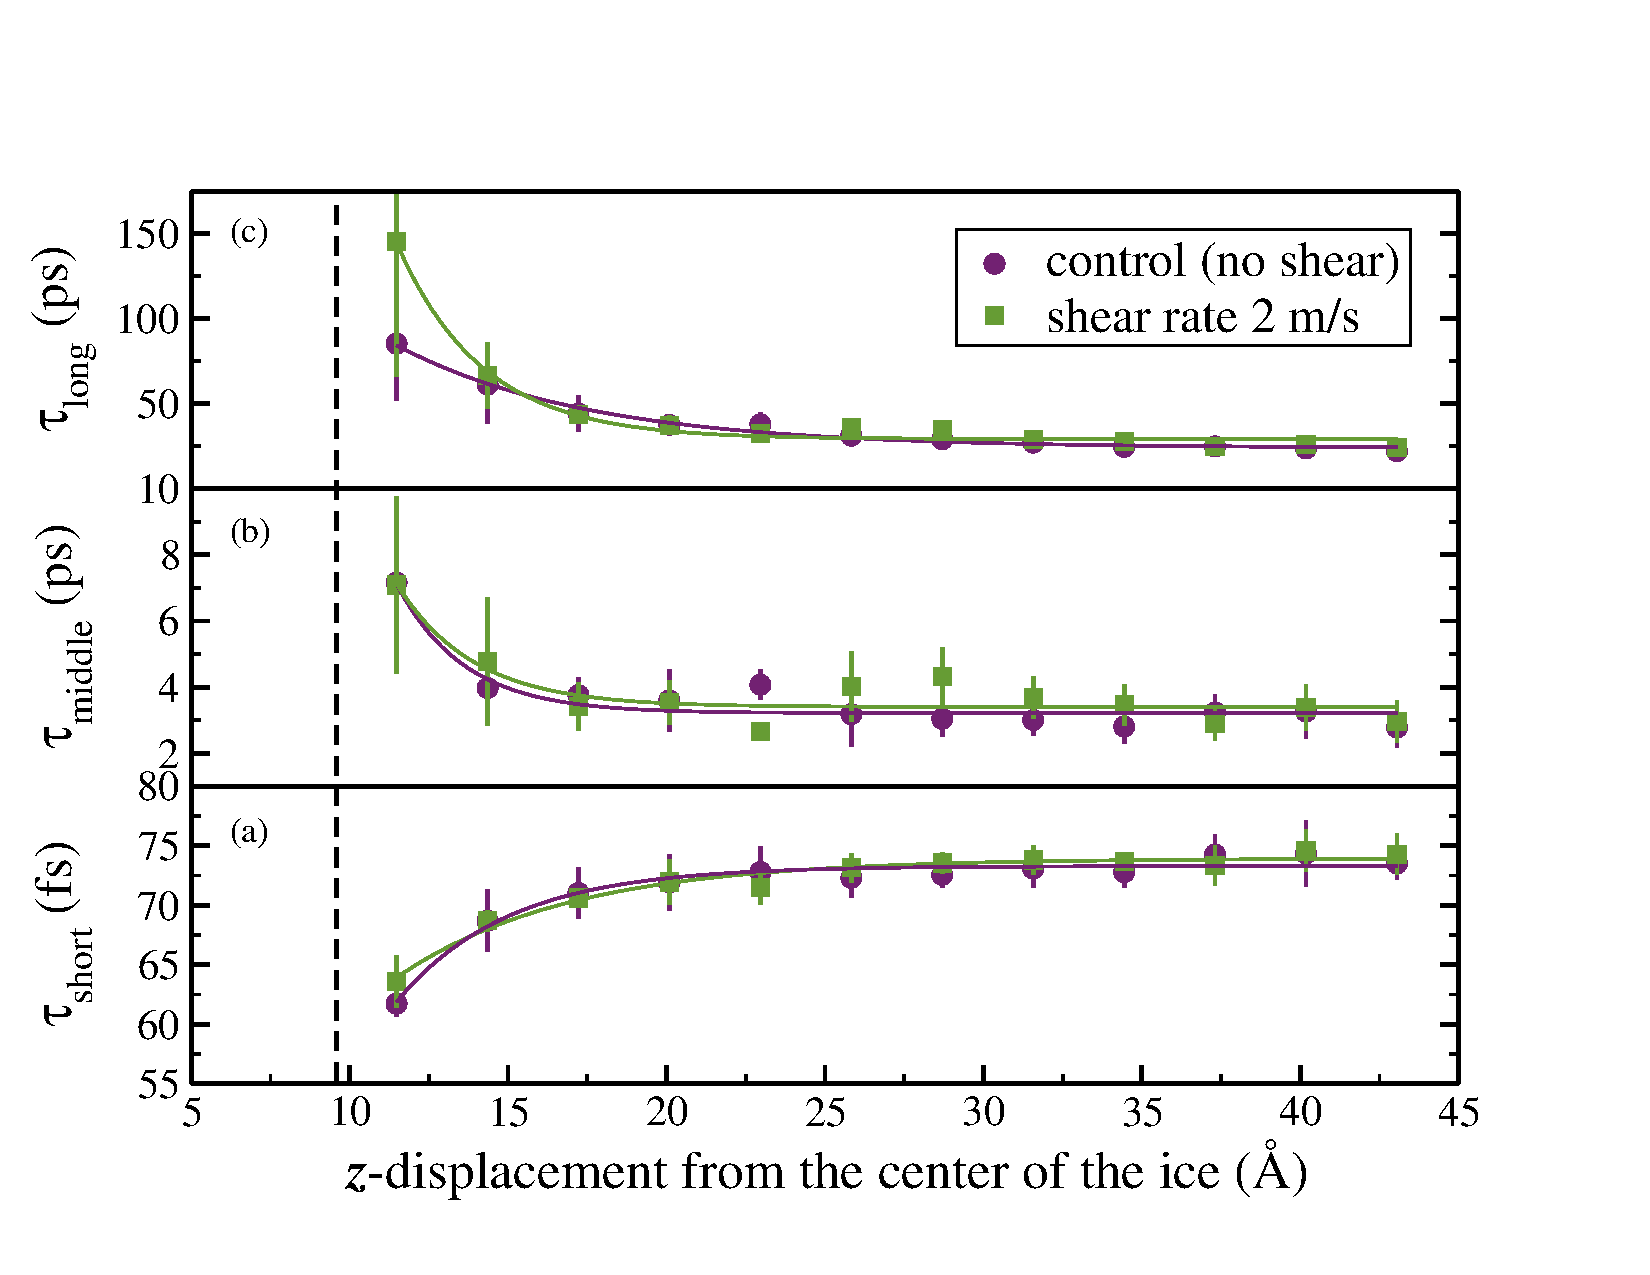
\includegraphics[width=\linewidth]{prismatic-orient}
\caption{\label{fig:Porient} Decay constants for $C_2(z,t)$ at the 
prismatic face. Panel descriptions match those in \ref{fig:PyrOrient}.}
\end{figure}


\end{document}
